\section{Misure di temperatura mediante termocoppia}
\paragraph{Dati e richieste}
Vengono fornite due serie di misure di temperatura allo scarico di una camera di combustione, eseguite mediante termocoppia di tipo B. La prima è costituita da 1599 valori ("Serie corta"), la seconda da 9999 ("Serie lunga"). Entrambe le serie sono campionate con una frequenza di campionamento di 100 Hz e vengono fornite mediante file testuale (.txt).\\
Si chiede di svolgere l'analisi statistica dei dati.
\subsection{Risoluzione}
Si riportano i risultati emersi dall'elaborazione dei dati sperimentali. I calcoli sono stati svolti mediante il software \textit{Matlab} e le funzioni built-in.
\paragraph{Suddivisione in classi e istogramma}
Entrambe le serie sono divise in 10 classi, di uguale ampiezza, costruite affinché non ci possa essere ambiguità nell'attribuzione dei valori: poiché le misure hanno 6 cifre decimali, gli estremi di classe sono definiti con 7 cifre decimali. L'estremo della prima classe viene scelto come il minimo valore di \glsxtrshort{symb:T} a cui viene sottratto 0.5e-7 \textsuperscript{o}C. Analogamente, l'estremo superiore dell'ultima classe viene calcolato sommando la stessa quantità al massimo valore di \glsxtrshort{symb:T} nella serie. I valori estremi delle due serie sono mostrati in Tab.\ref{tab:estremitemp}.
\begin{table} [H]
	\centering
	\begin{tabular}{c|c|c}
		\toprule
		\toprule
		\textbf{Serie} & \textbf{T\textsubscript{min} [\textsuperscript{o}C]} &\textbf{T\textsubscript{max} [\textsuperscript{o}C]} \\
		\midrule
		\midrule
		Corta & 953.745910 & 1193.110960\\
		\midrule
		Lunga & 931.352290 & 1449.917970 \\
		\bottomrule
		\bottomrule
	\end{tabular}
\caption{Valori estremi di temperatura}
\label{tab:estremitemp}
\end{table}
Gli istogrammi relativi alle due serie sono mostrati in Fig.\ref{fig:istboth}.
\begin{figure} [H]
	
	\begin{subfigure}{0.49\textwidth}
		\centering
		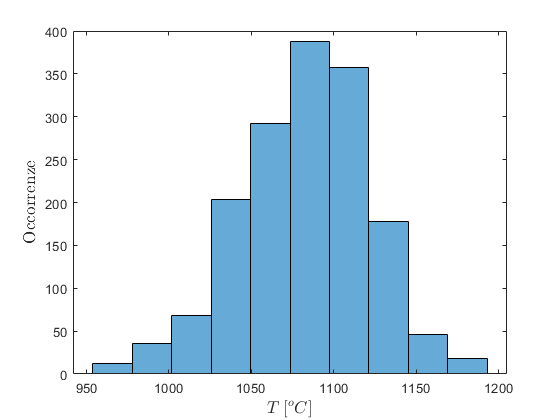
\includegraphics[width=0.99\linewidth]{chapters/1-misureT/istogrammashort}
		\caption{Serie corta}
		\label{fig:istogrammashort}
	\end{subfigure}%
	\begin{subfigure}{0.49\textwidth}
		\centering
		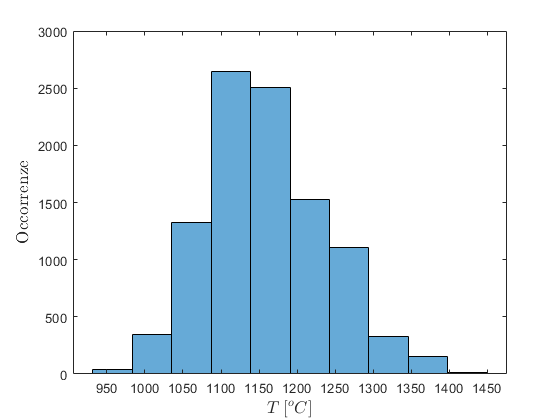
\includegraphics[width=0.99\linewidth]{chapters/1-misureT/istogrammalong}
		\caption{Serie lunga}
		\label{fig:istogrammalong}
	\end{subfigure}
\caption{Istogrammi delle due serie}	
\label{fig:istboth}
\end{figure}
AGGIUNGERE OSSERVAZIONI
